\documentclass[tikz,border=3mm]{standalone}
\usepackage[T1]{fontenc}
\usepackage[utf8]{inputenc}
\usepackage{lmodern}
\usetikzlibrary{arrows.meta,positioning,calc,shapes.geometric}
\definecolor{ink}{HTML}{202A33}
\definecolor{blue}{HTML}{2D7F9D}
\definecolor{orange}{HTML}{C97728}
\definecolor{light}{HTML}{B0C0D0}
\definecolor{soft}{HTML}{F3F5F7}
\begin{document}
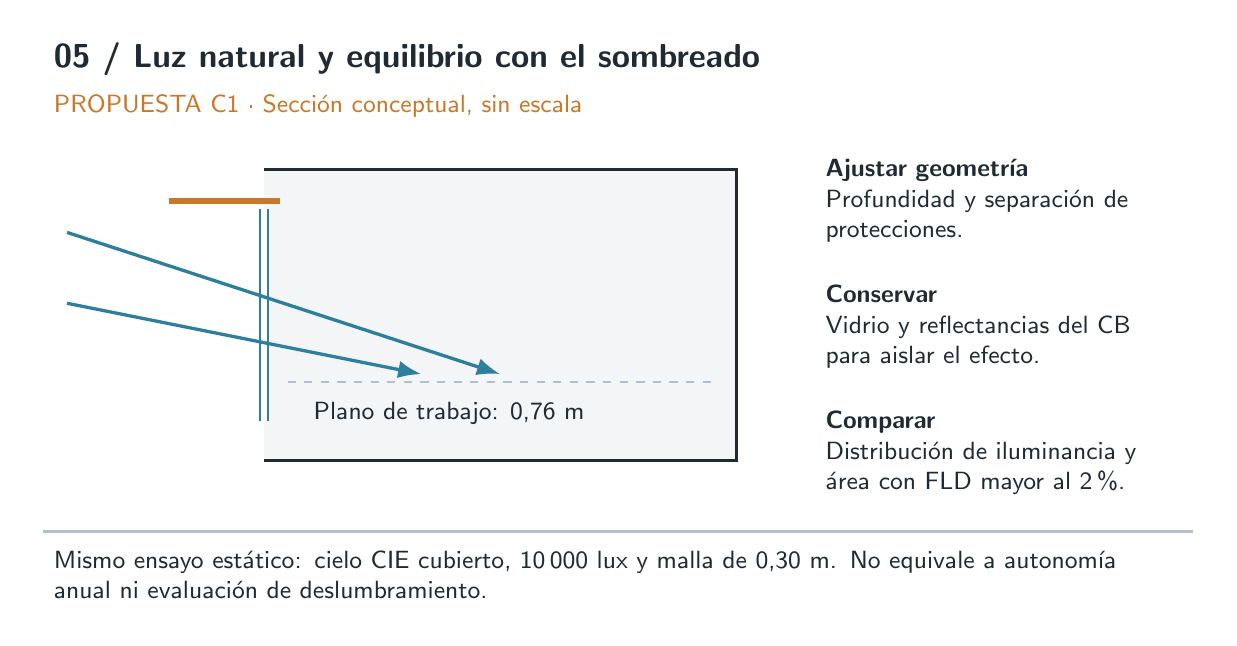
\begin{tikzpicture}[x=1cm,y=1cm,>=Latex,line width=.9pt,every node/.style={font=\sffamily\small,text=ink},note/.style={align=left,text width=4.1cm,anchor=west},flow/.style={->,blue,line width=1.2pt}]
\path[use as bounding box] (0,0) rectangle (15,7.5);


\node[anchor=west,font=\sffamily\bfseries\large] at (.2,7.1) {05 / Luz natural y equilibrio con el sombreado};
\node[anchor=west,text=orange] at (.2,6.5) {PROPUESTA C1 · Sección conceptual, sin escala};
\fill[soft] (3,2) rectangle (9,5.7);
\draw[ink] (3,2)--(9,2)--(9,5.7)--(3,5.7);
\draw[blue,double,double distance=2pt] (3,2.5)--(3,5.2);
\draw[orange,line width=2pt] (1.8,5.3)--(3.2,5.3);
\draw[flow] (.5,4.9)--(6,3.1);
\draw[flow] (.5,4)--(5,3.1);
\draw[light,dashed] (3.3,3)--(8.7,3);
\node[anchor=west] at (3.5,2.6) {Plano de trabajo: 0,76 m};
\node[note] at (10,5.3) {\textbf{Ajustar geometría}\\Profundidad y separación de protecciones.};
\node[note] at (10,3.7) {\textbf{Conservar}\\Vidrio y reflectancias del CB para aislar el efecto.};
\node[note] at (10,2.1) {\textbf{Comparar}\\Distribución de iluminancia y área con FLD mayor al 2\,\%.};
\draw[light] (.2,1.1)--(14.8,1.1);
\node[anchor=west,text width=14cm,align=left] at (.2,.55) {Mismo ensayo estático: cielo CIE cubierto, 10\,000 lux y malla de 0,30 m. No equivale a autonomía anual ni evaluación de deslumbramiento.};

\end{tikzpicture}
\end{document}
